\documentclass[10pt]{article}
\usepackage[letterpaper, margin=1in]{geometry}
\usepackage{fullpage}
% \usepackage[parfill]{parskip}    		% Activate to begin paragraphs with an empty line rather than an indent
\usepackage{graphicx}
\usepackage{amssymb}
\usepackage{wrapfig}
\usepackage{algorithm}
\usepackage{algpseudocode}
\usepackage{amsmath}
\usepackage{amsfonts}
\usepackage{listings}
\usepackage{url}
\usepackage{tikz}
\usetikzlibrary{calc,shapes.multipart,chains,arrows}
\usepackage{graphicx}
\usepackage{nameref}
\usepackage{xspace}
\usepackage{adjustbox}
\usepackage{framed}
\usepackage[all]{xy}
\usepackage{txfonts,pxfonts}
\usepackage{bm}
\usepackage{enumerate}
\usepackage{algorithm}
\usepackage{subfigure}
\usepackage{algpseudocode}
\usepackage[inference]{semantic}
\usepackage{paralist}
\usepackage[titletoc,title]{appendix}
\usepackage[english,printdayoff]{isodate}
\usepackage[pdftitle={PhD Proposal - Simone Atzeni}, pdfauthor={Simone
  Atzeni}, pdfsubject={PhD Proposal}]{hyperref}

\newcommand{\bigset}[2]{\big\{\;#1\;:\;#2\;\big\}}
\newcommand{\N}{\mathbb{N}}
\newcommand{\Z}{\mathbb{Z}}
\newcommand{\R}{\mathbb{R}}
\newcommand{\Np}{\mathbb{N^{+}}}

\title{\textbf{Low overhead data race detection in large structured parallel applications}}
%
\author{Simone Atzeni\\{\small simone@cs.utah.edu}}
%
\date{}

% \renewcommand*{\bibfont}{\footnotesize}

\lstset{language=C++,
  escapeinside=||,
  mathescape=true,
  basicstyle=\ttfamily,
  showstringspaces=false,
  keywordstyle=\color{blue}\ttfamily,
  stringstyle=\color{red}\ttfamily,
  % commentstyle=\color{green}\ttfamily,
  otherkeywords={\#pragma, omp, parallel, barrier, critical, num_threads, shared},
  breaklines=true,
  basicstyle=\small
}
  
\newenvironment{blockquote}{\par\medskip\leftskip=4em\rightskip=2em\noindent\ignorespaces}{\par\medskip}
% \newcommand*{\DEBUG}{}
\ifdefined\DEBUG
\newcommand{\simone}[1]{\todo[inline,size=\small, color=green!40]{S: #1}}
\else
\newcommand{\simone}[1]{}
\fi
\newcommand{\ganesh}[1]{\todo[inline,size=\small, color=yellow!40]{G: #1}}
\newcommand{\zvonimir}[1]{\todo[inline,size=\small, color=blue!40]{Z: #1}}
\newcommand{\dong}[1]{\todo[inline,size=\small, color=red!40]{D: #1}}
\newcommand{\ignacio}[1]{\todo[inline,size=\small, color=yellow!40]{I: #1}}
\newcommand{\greg}[1]{\todo[inline,size=\small, color=yellow!40]{L: #1}}
\newcommand{\martin}[1]{\todo[inline,size=\small, color=yellow!40]{M: #1}}

\newcommand{\archer}{\textsc{Archer}\xspace}
\newcommand{\tsan}{TSan\xspace}
\newcommand{\iomp}{Intel\circledR OpenMP* Runtime\xspace}
\newcommand{\omp}{LLVM OpenMP Runtime\xspace}
\newcommand{\insp}{Intel\circledR Inspector XE\xspace}
\newcommand{\amg}{AMG2013\xspace}

%%% Local Variables:
%%% mode: latex
%%% eval: (flyspell-mode 1)
%%% TeX-master: "root.tex"
%%% End:


\begin{document}

\maketitle

\section{Introduction}
\label{sec:introduction}

Multithreaded programming has become widespread in use, given the need to
employ multicore CPUs to gain higher performance at a given energy budget.
%
In the High Performance Computing (HPC) world, this has lead to an increased
adoption of on-node parallelism in large software applications.
%
This trend is confirmed by work that is in progress at national research
facilities~\cite{sierra, summit, trinity}.

Multithreaded programming is achieved through different programming models
(e.g. Pthreads); however, the predominant paradigm of choice in HPC is
OpenMP~\cite{ompdoc}, which guarantees portability and ease of use.
%
In fact, we are collaborating with computational scientists at the Lawrence
Livermore National Laboratory (LLNL), one of the world's largest computing
facilities, where one of the main ongoing tasks is the porting of critical
multiphysics application~\cite{llnl-apps} to OpenMP.
%
In this community, OpenMP is of paramount importance to enable shared memory
parallel programming; yet, porting large HPC applications to OpenMP is
error-prone.
%
The correctness of these applications is crucial to the reliability of
critical simulations pertaining to many real world phenomena of fundamental
importance such as modeling of nuclear explosions, weather simulations,
hydrodynamics modeling, etc.
%
One of the most common of error types in OpenMP applications is data
races~\cite{sus_common_2008}.
%
Data races are often hard to locate with traditional debugging methods.
%
Fast and precise checking tools to detect data races are needed now more than
ever.
%
While data race is a well-known problem and many Pthreads data race detection
tools have been proposed over the past twenty years, none or just a few of
them are actually able to analyze OpenMP programs.
%
Our work targets this critical need.

Data race detection research has focused both on static and dynamic analysis
techniques.
%
Static analysis techniques allow to reason about all the inputs of the program
and the interleavings of the threads, and they are fairly scalable and fast
since no runtime overhead is incurred.
%
However, the lack of information that exists only at runtime makes these
techniques very imprecise; in fact they often miss races and generate many
false positives.
%
Runtime techniques are precise, as they do not report any false positives, and
only report races in the branches of programs that are actually executed.
%
On the other hand dynamic analysis for data race detection is known to
generate a very high runtime and memory overhead due to the operations it
needs to perform and the states it needs to maintain during the execution.

The runtime overhead of even the best of dynamic tools, such as the
ThreadSanitizer (Tsan) and Intel Inspector XE, can cause between $5x-20x$
slowdown and the memory overhead can be between $2x-10x$ of the memory used by
the normal execution of the programs.
%
For very large programs, such as HPC applications, the runtime and memory
overheads can be even bigger.
%
For instance, our experiments show that this slowdown can be $100x$
and the memory consumption can be $50x$ larger.
%
The high runtime slowdown and memory usage make such tools useless from the
point of view of actual developers, who probably would not be keen on waiting
a long time to check their programs; or they may not even have enough machine
resources to run the tools.
%
We definitely need better techniques -- static, dynamic, or combinations -- to
detect data races in large structured parallel applications.

\subsection{Thesis statement}
\label{subsec:statement}

The goal of this dissertation is to provide an approximate but fast data race
detection tool for large OpenMP applications that combine static and dynamic
analysis.
%
\emph{Our thesis statement is that by combining the best of these techniques
  and tailoring the implementation to the actual concurrency structure of
  structured parallel languages such as OpenMP, we can make data race checking
  of HPC applications practical.}

Our approach is now briefly summarized.
%
First, we combined static and existing dynamic techniques to reduce the amount
of code to analyze at runtime, thus lowering the overheads.
%
As we will show in \S~\pageref{sec:accomplishedwork}, the first approach allow
in general a speed up of about 25\%, which is still not enough for large HPC
applications.
%
Therefore as second approach, we will develop a new runtime technique for data
race detection that exploits the structured parallelism of OpenMP to reduce
runtime and memory overhead.
%
In order to guarantee a fast data race detection, we give up some precision
and accuracy which only produce more false positives but still guarantee the
absence of false negatives.
%
Furthermore, we provide to the user a mechanism to further check part of all
the reported races with a more precise data race detection techniques (e.g
Tsan).
%
This approach will allow to speedup the more precise race detection
techniques since the runtime check will only focus on a smaller amount of
memory accesses.
%
Our project goals are now listed, as conceived at the beginning of our
research.

\begin{itemize}
\item \textbf{Sequential Blacklisting:} We will design a static analysis to
  identify the code executed sequentially in a OpenMP program.
\item \textbf{Data Dependency Analysis:} We will design a static analysis
  technique that identify race free code in a OpenMP program to exclude it
  from the runtime analysis.
\item \textbf{\archer v1:} We will combine the static analysis with the
  existing Clang/LLVM Tsan data race detection tool and we will make Tsan
  capable of detect data races in OpenMP programs, as part of a first version
  of a data race detector called \archer.
\item \textbf{Clock-less runtime algorithm:} We will design and implement a
  new runtime analysis technique that exploits the structured parallelism of
  the OpenMP paradigm in order to reduce the runtime and memory overheads.
\item \textbf{\archer v2:} We will embed the aforementioned new runtime
  technique in a second version of \archer as a replacement of the \tsan
  runtime.
\end{itemize}

The first three goals have been achieved in our previous
workshop~\cite{Protze:2014:TPL:2688361.2688369} and
conference~\cite{atzeni2016} papers.

%%% Local Variables:
%%% mode: latex
%%% eval: (flyspell-mode 1)
%%% TeX-master: "root.tex"
%%% End:

\section{Background}
\label{sec:background}

\begin{itemize}
\item Existing techniques
\item Happens-before
\item Lock-set
\item Hybrid
\item Pros and cons
\item Thread-sanitizer
\item Pros and cons
\end{itemize}

%%% Local Variables:
%%% mode: latex
%%% eval: (flyspell-mode 1)
%%% TeX-master: "root.tex"
%%% End:

\section{Proposed Research}
\label{sec:proposedresearch}

To motivate the need for better data race detection techniques for structured
parallelism (i.e. OpenMP), rather than classic techniques such as
happens-before relation, consider the example in Figure~\ref{fig:nested}.
%


\begin{figure}
  \centering
  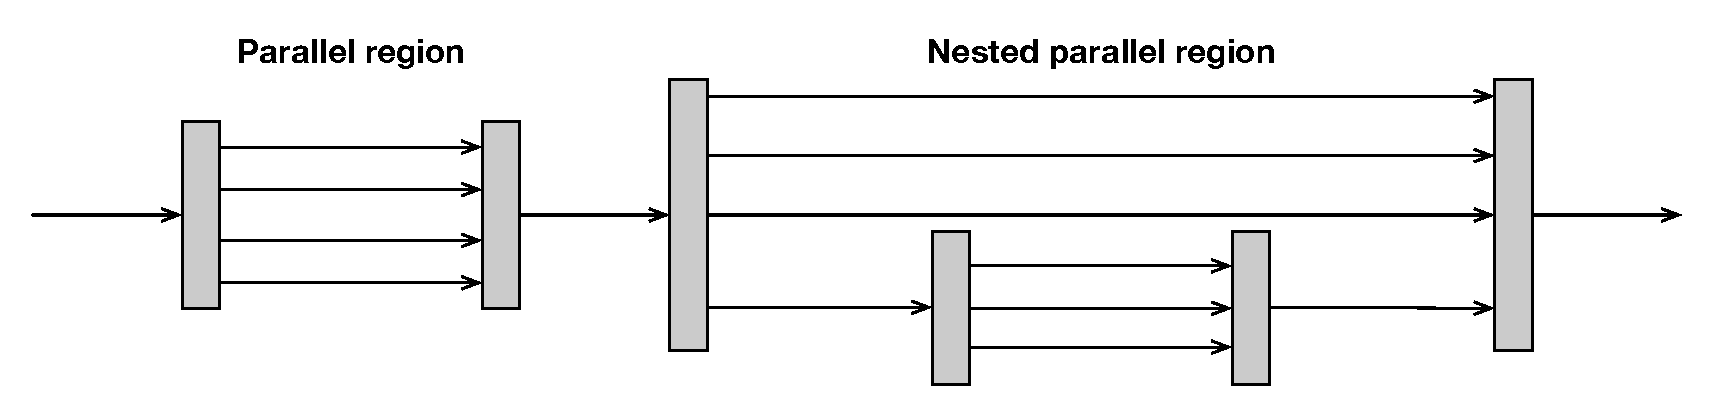
\includegraphics[width=0.95\textwidth]{figures/nested_parallelism}
  \caption{OpenMP nested parallelism}
  \label{fig:nested}
\end{figure}

\begin{itemize}
\item Static + dynamic analysis
\item Sequential blacklisting due to OpenMP structured parallelism
\item Barrier intervals
\item labeling to identify concurrent threads
\item sort of lock-set
\item Implemented by central but fast data structure
\item OMPT/OMPD
\end{itemize}

%%% Local Variables:
%%% mode: latex
%%% eval: (flyspell-mode 1)
%%% TeX-master: "root.tex"
%%% End:

\section{Accomplished Work}
\label{sec:accomplishedwork}

The first part of the work has been accomplished and published
in~\cite{Protze:2014:TPL:2688361.2688369, atzeni2016}.
%

%
I have worked 

\begin{itemize}
\item Archer Paper
\item Static + dynamic
\item Data dependency analysis
\item Sequential blacklisting
\item Current improvement in runtime and memory overhead
\end{itemize}

%%% Local Variables:
%%% mode: latex
%%% eval: (flyspell-mode 1)
%%% TeX-master: "root.tex"
%%% End:

\section{Timeline}
\label{sec:timeline}

\begin{enumerate}
\item \textbf{November 2014:} Presented paper at LLVM-HPC Workshop 2014 at SC
  2014.
\item \textbf{May 2016:} Present paper on \archer v1 at IPDPS 2016.
\item \textbf{July 2016:} Submit paper to POPL 2017, or PPoPP 2017.
  % 
  We aim for a first version of the proposed runtime algorithm.
\item \textbf{Septmber -- February 2017:} Release final version of \archer
  (combination of static analysis and new runtime) with extensive evaluation
  of the tool on large HPC benchmarks.
  %
  Sumbit it to PLDI, IPDPS, CGO, or PACT.
\item \textbf{May 2017:} Submit PhD dissertation.
\end{enumerate}

%%% Local Variables:
%%% mode: latex
%%% eval: (flyspell-mode 1)
%%% TeX-master: "root.tex"
%%% End:


\bibliographystyle{abbrv}
\bibliography{references}

\newpage
\begin{appendices}
  \section{OpenMP Concurrency Operational Semantics}
\label{sec:appendixa}

\subsection{Convention}
\label{subsec:convention}

\begin{compactitem}
\item $\N$ is the set of natural numbers, $\{0,1,2,\ldots\}$.
\item $x\in\N$ can be treated as a set $\{0,\ldots,x-1\}$ as in set theory.
  Thus, $0=\{\}$, $1=\{0\}$, $2=\{0,1\}$, $3=\{0,1,2\}$, etc.
  %
  This is standard in set-theory (usage courtesy of Milner).
  %
  Whenever we treat a member of $\N$ as a number as well as a set, we'll make
  sure to provide a hint.
\item $t\in TID$ is a thread ID (a natural number) for some $TID\in \N$ ($TID$
  thread IDs are allowed).
\item Let $ADDR\in\N$ be the range of memory addresses accessed by the various
  threads.
\end{compactitem}

\subsection{Offset-Span Labels}
\label{subsec:osl}

We follow the concept of offset-span labels introduced in the paper of
Mellor-Crummey~\cite{Mellor-Crummey:1991:ODD:125826.125861}.
%
An offset-span label ($osl$ for short) labels each thread's execution point
with a sequence of pairs, marking its lineage in the concurrency structure
defined by prior forks and joins.
%
The domain of $OSL = ((\N\times\N))^{\N}$, i.e. each member $osl\in OSL$ is a
sequence of pairs
\[ \langle a_1,b_1\rangle, \langle a_2,b_2\rangle,\ldots,\langle
a_n,b_n\rangle\] suppose $osl_1, osl_2\in OSL$.
%
These labels are sequential exactly when one of the OSLs (say $osl_1$) is a
prefix of the other.
%
Other wise, they are concurrent.
%
For further details, please see~\cite{Mellor-Crummey:1991:ODD:125826.125861}.

\subsection{System State}
\label{subsec:systemstate}

The state of the system consists of a global states $GS$ and a set of thread
local states $TP$ (Thread Pool).
%
The total state $ts$ of any system is a pair ``Global State, Thread Pool;''
i.e., a specific total state $ts$ is:
\[ ts = \langle gs, tp \rangle \]
\noindent Each total state $ts$ comes from the domain $T$S, where
$TS = GS\times TP$.

\noindent Each global state $gs$ is a 5-tuple:
\[ \langle bm, m, n, rw, \sigma \rangle \]
\noindent Each global state $gs$ comes from the domain $GS$, where
\[ TS = BM\times M\times N\times RW\times \Sigma \]

\noindent where:
%
\begin{compactitem}
\item The domain $BM = ParRegID \mapsto (\N\times \N)$.  Thus, for each
  $bm\in BM$, we have $bm\; :\; ParRegID \mapsto (\N\times \N)$.
  %
  Given a $p\in ParRegID$, $bm$ returns a pair of natural numbers $(a,b)$,
  where $a$ is the ``current Barrier Count'' and $b$ is the ``target Barrier
  Count.''
  %
  When a thread $t$ with offset span label $osl$ executes a $ParBegin(N)$
  instruction, $N$ threads are created, and an entry
  $\langle osl, (0,N)\rangle$ is added to function $bm$\footnotemark.
  %
  \footnotetext{Recall that functions are single-valued relations, or sets of
    pairs with unique second component for each given first component.  Thus,
    $\{\langle osl,(0,N)\rangle\}$ is a function. We will allow functions to
    evolve, i.e. undefined for items explicitly added.}
  %
  The first field $0$ will be incremented each time we close a barrier or a
  parallel region, in a manner to be described momentarily.
  %
  Threads that have to meet a barrier or have to hit the $ParEnd$ constructs.

\item Mutex $m$ comes from domain $M$, where $M=\{-1\}\cup \N$.  Each $m$ is
  initialized to $-1$ when the mutex is free.
  %
  When thread $t\in TID$ acquires the mutex, we record the value $t$ in $m$,
  indicating that the mutex is taken, and also taken by which thread.

\item ``Nutex'' $n$ comes from domain $N$ where
  $N = Names \mapsto (\{-1\} \cup TID)$.
  %
  That is, given a named mutex name $n \in Names$, $N[n] = -1$ means that this
  named mutex (``nutex'') is free.
  %
  Otherwise, $N[n] = t$, recording the fact that this nutex is held by thread
  $t$.

\item Let memory access-type $MAT=\{R,W\}$.

\item $rw\in RW$ is a tuple that maintains all the memory accesses of each
  thread in the system.
  %
  We have
  $RW = TID\times OSL \times \N \times ADDR \times MAT \times M\times N$.
  %
  Each memory access performed by thread $t$ is recorded as the tuple
  \[ \langle tid, osl, bl, addr, mat, mutex, nutex \rangle \] where:
  \begin{compactitem}
  \item $tid\in TID$ is the thread ID;
  \item $osl\in OSL$ is the offset-span label;
  \item $bl\in \N$ is the barrier label of the last barrier seen by the thread
    $t$;
  \item $addr\in ADDR$ is the memory address;
  \item $type\in\{R,W\}$ records reads or writes;
  \item $mutex$ is the mutex state (value of $M$ in $GS$) at the time of the
    access;
  \item $nutex$ is the nutex state (value of $N$ in $GS$) at the time of the
    access.
  \end{compactitem}

\item $\sigma\in\Sigma$ is the data state of the system, as described earlier.
\end{compactitem}

\vspace{2ex}

The local state $TP$ is the thread pool that contains a list of 3-tuples, each
of which is the local state of a thread:
\[ \langle tid, osl, bl \rangle \]

The domain $TP=2^{TID\times OSL\times \N}$ where:

\begin{compactitem}
\item $t\in TID$ is thread ID of the thread;
\item $osl\in OSL$ is an offset-span label;
\item $bl\in\N$ is the label of the barrier the thread has witnessed last.
  %
  We assume that each barrier instruction is of the form $bar(L)$ where
  $L\in\N$ carries the barrier number.
  %
  A thread crossing a barrier sets its $bl$ to the value $L$.
\end{compactitem}

\subsection{Helper Functions and Predicates}
\label{subsec:helper}

\begin{compactitem}
\item $as$: is used as in Ocaml (it allows a name for a whole structure, as
  well as helps us refer to the inner details of the structure).
\item $most(lst)$: we define $most$ as a function that return the same list
  given in input except the last element (i.e. in Python lst[:-1]).
\item $\parallel$: This operator is used to describe that two different
  threads are concurrent.
  %
  In particular, given two offset-span labels $l1$ and $l2$, $l1 \parallel l2$
  (read $l1$ and $l2$ are concurrent) means that the two threads associated to
  the two offset-span labels are concurrent.
  %
  In case the labels represent barrier labels, it means that the two barrier
  are concurrent, in other words they happen in two different (nested)
  parallel regions.
\item $SpawnChildren(\langle ptid, posl, pbl \rangle, \sigma, N)$: Given the
  parent's TID ($ptid$), offset-span label ($posl$) and barrier label ($pbl$),
  this function creates a pool of $N$ threads -- specifically, the local
  states of these threads $\langle tid, osl, bl \rangle$.
  %
  It initializes the offset-span label $osl$ for each thread created using the
  rules in \S\ref{sec:osl}, by extending $posl$ with pairs $[0,N]$ through
  $[N-1,N]$.
  %
  The $bl$ is set to $pbl$.
  %
  The TIDs are somehow uniquely generated ($osl$ could be used as an index
  into an evolving TID bijection).
\item $GetChildJoin(tp)$: returns the single thread-state triple that results
  from fusing all the threads in the thread pool $tp$.
  %
  The offset-span labels are all chopped, and the single data state that is
  carried forward has the right PC and data state, going forward.
\item $Concurrent(OSL, t1, t2)$ is as described in \S\ref{sec:osl}.
\item Function $AddRW(\langle tid, osl, bl, addr, mat, m, n \rangle)$ adds the
  access into the RW Structure.
  %
  The record says ``an access by $tid$ with offset-span label $osl$ and
  barrier label $bl$ is performed at address $addr$ with memory access type
  $mat$, when the mutex state is $m$ and the nutex state is $n$.''
\item $Full(bm, osl)$: This predicate keeps the counts the number of threads
  that have reached a $ParEnd(N)$ (or a $Barrier(bid)$) construct.
  %
  In order to count the threads, it uses the structure $bm$ which is indexed
  by the $ParRegID$ represented by the offset-span label $osl$.
  %
  In other word, the predicate $Full$ means that other threads have reached
  the construct and have incremented the counter in the $bm$ structure.
  %
  From a functional language point of view $Full$ would look like:

  \begin{center}
    \lstset{language=[Objective]Caml}
    \begin{lstlisting}
      let Full(bm, osl) =
         let (count, N) = bm[osl]
         in (count == N - 1)
    \end{lstlisting}
  \end{center}
\end{compactitem}

\subsection{Structured Operational Semantics Rules}
\label{sec:sosrules}

\begin{framed}
  \[
  \inference[ParBegin(N)]{
    gs\; {\rm as}\; (bm, m, n, rw, \sigma) \in GS \\
    te\; {\rm as}\; (tid, osl, bl) \in TP \\
    at(tid, \sigma, ParBegin(N)) \\
    tp' = (tp - \{te\} \cup SpawnChildren(\langle tid, osl, bl \rangle, \sigma, N))\\
    bm' = bm \cup \{\langle osl,(0,N)\rangle\}\\
    \sigma' = nxt(\sigma, tid)
  }
  {\langle gs, tp \rangle \longrightarrow
    \langle gs'\; {\rm as}\; \langle bm',m,n,rw,\sigma'\rangle, tp' \rangle
  }
  \]
  
  \[
  \inference[ParEnd(N)]{
    gs\; as\; (bm, m, n, rw, \sigma) \in GS \\
    te\; as\; (tid, osl, bl) \in TP \\
    tp' \subseteq tp \\
    at(tid, \sigma, ParEnd(N)) \\
    Full(bm, most(osl)) \\
    bm' = bm - \{\langle most(osl), * \rangle\} \\
    \sigma' = nxt(\sigma, tid) \\
    tp'' = tp - tp' \cup GetChildJoin(tp')}
  {\langle gs, tp \rangle \longrightarrow
    \langle gs'\; {\rm as}\; \langle bm',m,n,rw,\sigma'\rangle, tp'' \rangle
  }
  \]

  \[
  \inference[ParEnd(N)]{
    gs\; as\; (bm, m, n, rw, \sigma) \in GS \\
    te\; as\; (tid, osl, bl) \in TP \\
    tp' \subseteq tp \\
    at(tid, \sigma, ParEnd(N)) \\
    \neg Full(bm, most(osl)) \\
    bm[most(osl)]\; as\; (count, N) \\
    bm' = bm \cup \{\langle osl,(count+1,N) \rangle\} \\
    \sigma' = nxt(\sigma, tid)}
  {\langle gs, tp \rangle \longrightarrow \langle gs'\; {\rm as}\; \langle bm',m,n,rw,\sigma'\rangle, tp \rangle}
  \]

  \[
  \inference[AcquireMutex]{
    gs\; as\; (bm, m, n, rw, \sigma) \in GS \\
    te\; as\; (tid, osl, bl) \in TP \\
    at(tid, \sigma, AcquireMutex()) \\
    m = -1 \\
    m' = tid \\
    \sigma' = nxt(\sigma, tid)}
  {\langle gs, tp \rangle \longrightarrow \langle gs'\; {\rm as}\; \langle bm,m',n,rw,\sigma' \rangle, tp \rangle}
  \]

  \[
  \inference[ReleaseMutex]{
    gs\; as\; (bm, m, n, rw, \sigma) \in GS \\
    te\; as\; (tid, osl, bl) \in TP \\
    at(tid, \sigma, ReleaseMutex()) \\
    m = t \\
    m' = -1 \\
    \sigma' = nxt(\sigma, tid)}
  {\langle gs, tp \rangle \longrightarrow \langle gs'\; {\rm as}\; \langle bm,m',n,rw,\sigma' \rangle, tp \rangle}
  \]

  \[
  \inference[AcquireNutex(name)]{
    gs\; as\; (bm, m, n, rw, \sigma) \in GS \\
    te\; as\; (tid, osl, bl) \in TP \\
    at(tid, \sigma, AcquireNutex(name)) \\
    n[name] = -1 \\
    n' = n[name \rightarrow tid] \\
    \sigma' = nxt(\sigma, tid)}
  {\langle gs, tp \rangle \longrightarrow \langle gs'\; {\rm as}\; \langle bm,m,n',rw,\sigma' \rangle, tp \rangle}
  \]

  \[
  \inference[ReleaseNutex(name)]{
    gs\; as\; (bm, m, n, rw, \sigma) \in GS \\
    te\; as\; (tid, osl, bl) \in TP \\
    at(tid, \sigma, ReleaseNutex(name)) \\
    n[name] = tid \\
    n' = n[name \rightarrow -1] \\
    \sigma' = nxt(\sigma, tid)}
  {\langle gs, tp \rangle \longrightarrow \langle gs'\; {\rm as}\; \langle bm,m,n',rw,\sigma' \rangle, tp \rangle}
  \]

  \[
  \inference[LoadStore]{
    gs\; as\; (bm, m, n, rw, \sigma) \in GS \\
    te\; as\; (tid, osl, bl) \in TP \\
    at(tid, \sigma, LoadStore(addr, mat)) \\
    rw' = AddRW(tid, osl, bl, addr, mat, mutex, nutex) \\
    \sigma' = nxt(\sigma, tid)}
  {\langle gs, tp \rangle \longrightarrow \langle gs'\; {\rm as}\; \langle bm,m,n,rw',\sigma' \rangle, tp \rangle}
  \]

  \[
  \inference[Barrier(bid)]{
    gs\; as\; (bm, m, n, rw, \sigma) \in GS \\
    te\; as\; (tid, osl, bl) \in TP \\
    at(tid, \sigma, Barrier(bid)) \\
    Full(bm, most(osl)) \\
    bm' = bm - \{\langle osl,* \rangle\} \\
    \sigma' = nxt(\sigma, tid)}
  {\langle gs, tp \rangle \longrightarrow
    \langle gs'\; {\rm as}\; \langle bm',m,n,rw,\sigma'\rangle, tp \rangle
  }
  \]

  \[
  \inference[Barrier(bid)]{
    gs\; as\; (bm, m, n, rw, \sigma) \in GS \\
    te\; as\; (tid, osl, bl) \in TP \\
    at(tid, \sigma, Barrier(bid)) \\
    \neg Full(bm, most(osl)) \\
    bm[most(osl)]\; as\; (count, N) \\
    te' as (tid, osl, bid) \\
    tp' = tp - te \cup \{ te' \} \\
    bm' = bm \cup \{\langle osl,(count+1,N) \rangle\} \\
    \sigma' = nxt(\sigma, tid)}
  {\langle gs, tp \rangle \longrightarrow \langle gs'\; {\rm as}\; \langle bm',m,n,rw,\sigma'\rangle, tp' \rangle}
  \]

  \[
  \inference[Barrier(bid)]{
    gs\; as\; (bm, m, n, rw, \sigma) \in GS \\
    te_1\; as\; (tid_1, osl1, bl1) \in tp\\
    te_2\; as\; (tid_1, osl1, bl1) \in tp \\
    (tid_1 \neq tid_2) \\
    Concurrent(osl, tid_1, tid_2) \\
    i \in rw[tid_1] \\
    j \in rw[tid_2] \\
    (rw[tid_1][i].addr == rw[tid_2][j].addr) \\
    (rw[tid_1][i].mat == W) \vee (rw[tid_2][j].mat == W) \\
    (rw[tid_1][i].mutex == -1) \vee (rw[tid_2][j].mutex == -1) \\
    (rw[tid_1][i].nutex \cap rw[tid_2][j].nutex = \emptyset) \\
    (rw[tid_1][i].bl == rw[tid_2][j].bl) \vee (rw[tid_1][i].bl \parallel rw[tid_2][j].bl)}
  {\langle gs, tp \rangle \rightarrow RaceFail(\sigma, addr, tid_1, tid_2)}
  \]
\end{framed}

%%% Local Variables:
%%% mode: latex
%%% eval: (flyspell-mode 1)
%%% TeX-master: "root.tex"
%%% End:

\end{appendices}

\end{document}

%%% Local Variables:
%%% mode: latex
%%% eval: (flyspell-mode 1)
%%% TeX-master: "root.tex"
%%% End:
